% Overleaf: Compiler = XeLaTeX; Main document = main.tex
% 圖片直接以 Pianists.png 呼叫，請與 main.tex 放在同一層；不需圖片資料夾或 .bib 檔。
\documentclass[UTF8,12pt,a4paper,fontset=none]{ctexart}

% Compiler: XeLaTeX。停用 Fandol，明確指定繁體中文字型與字重。
% 中文斜體維持正體字形；英文斜體由西文字型負責。
\setCJKmainfont[
  UprightFont = *,
  BoldFont = * Bold,
  ItalicFont = *,
  BoldItalicFont = * Bold
]{Noto Serif CJK TC}
\setCJKsansfont[
  UprightFont = *,
  BoldFont = * Bold,
  ItalicFont = *,
  BoldItalicFont = * Bold
]{Noto Sans CJK TC}
\setCJKmonofont[
  UprightFont = *,
  BoldFont = * Bold,
  ItalicFont = *,
  BoldItalicFont = * Bold
]{Noto Sans CJK TC}
\AtBeginDocument{\renewcommand{\contentsname}{目錄}}

\usepackage[margin=2.2cm,headheight=16pt]{geometry}
\usepackage{fontspec}
\setmainfont{TeX Gyre Termes}
\usepackage{setspace,xcolor,graphicx,booktabs,tabularx,array,enumitem}
\usepackage[most]{tcolorbox}
\usepackage{fancyhdr,tikz,longtable}
\usepackage[colorlinks=true,linkcolor=teal!65!black,urlcolor=teal!65!black]{hyperref}
\hypersetup{unicode=true,bookmarksnumbered=true,pdftitle={黑白極致・巨擘對話：音樂會導聆},pdfauthor={個人聆聽手冊}}
\definecolor{ink}{HTML}{24333D}
\definecolor{accent}{HTML}{2B6869}
\definecolor{paper}{HTML}{F3F5F2}
\definecolor{gold}{HTML}{A57A43}
\onehalfspacing
\setlength{\parindent}{2em}
\setlength{\parskip}{4pt}
\setlist[itemize]{leftmargin=1.6em,itemsep=3pt,topsep=3pt}
\ctexset{section={format=\Large\bfseries\color{accent}},subsection={format=\large\bfseries\color{ink}}}
\newtcolorbox{listen}[1]{enhanced,breakable,colback=paper,colframe=accent!30,boxrule=0.5pt,arc=1mm,title=#1,colbacktitle=accent,coltitle=white,fonttitle=\bfseries,left=3mm,right=3mm}
\newcommand{\src}[1]{{\small\color{accent}[資料 #1]}}
\newcommand{\work}[2]{\textbf{#1}\par{\small\itshape #2}\par}
\pagestyle{fancy}\fancyhf{}
\fancyhead[L]{\small 黑白極致・巨擘對話}
\fancyhead[R]{\small 2026.11.07・新竹}
\fancyfoot[C]{\thepage}
\setlength{\emergencystretch}{3em}
\raggedbottom
\renewcommand{\arraystretch}{1.12}
\begin{document}
\begin{titlepage}
\color{ink}
\vspace*{0.4cm}
{\large\sffamily 2026\quad HSINCHU}\par
\vspace{0.7cm}
{\Huge\bfseries 黑白極致}\par\vspace{0.25cm}
{\Huge\bfseries 巨擘對話}\par
\vspace{0.7cm}
{\LARGE 名家音樂會導聆}\par
\vspace{0.2cm}
{\large Two Pianos, Many Voices}\par
\vspace{0.65cm}
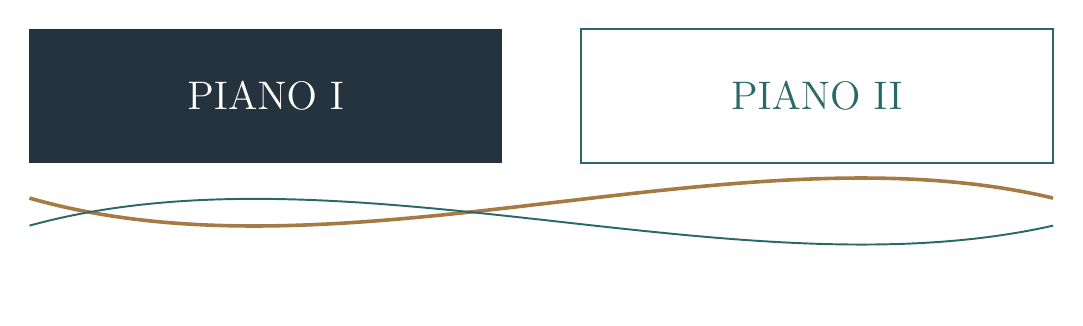
\begin{tikzpicture}[x=1cm,y=1cm]
\fill[ink] (0,0) rectangle (6,1.7);
\draw[accent,line width=0.8pt] (7,0) rectangle (13,1.7);
\node[text=white,font=\Large] at (3,0.85) {PIANO I};
\node[text=accent,font=\Large] at (10,0.85) {PIANO II};
\draw[gold,line width=1.3pt] (0,-0.45) .. controls (4,-1.6) and (9,0.5) .. (13,-0.45);
\draw[accent,line width=0.7pt] (0,-0.8) .. controls (4,0.3) and (9,-1.7) .. (13,-0.8);
\end{tikzpicture}
\vspace{0.8cm}
{\large 2026 年 11 月 7 日（星期六）14:30}\par
新竹市文化局演藝廳音樂廳\par
新竹市北區東大路二段 17 號\par
\vspace{0.6cm}
\textbf{嚴俊傑・盧易之・汪奕聞・Peter Ovcharov}\par
\vfill
{\small 史坦威開琴系列活動・個人聆聽手冊\\
依公開資料整理，查核日期：2026 年 11 月 1 日。\\
曲序、樂章選擇、改編版本與演出分工，以現場節目單為準。}
\end{titlepage}
\tableofcontents
\clearpage
\section{先看這場音樂會的輪廓}
這場音樂會以雙鋼琴與八手聯彈為主，由四位鋼琴家合作演出。兩台琴有時輪流接續旋律，有時分別負責低音、和聲與節奏；四人一起演奏時，聲部也更豐富。除了欣賞各人的演奏，也可以留意他們如何配合，讓不同的聲音清楚地結合在一起。

本手冊聚焦 11 月 7 日的名家音樂會，演奏家為嚴俊傑、盧易之、汪奕聞與 Peter Ovcharov。\src{1} 以下按作品編排導聆，並非正式曲序。

\begin{listen}{已公布的節目資訊}
售票頁列有莫札特 K.448、德布西《黑與白》、拉威爾《圓舞曲》，以及《土耳其狂想曲》《骷髏之舞》的八手聯彈。巴赫與拉赫曼尼諾夫也在介紹中，但尚未列出曲名。各曲的演奏搭檔與八手版本改編者，以正式節目單為準。\src{1}
\end{listen}

\begin{tabularx}{\textwidth}{@{}p{0.24\textwidth}X@{}}
\toprule
\textbf{作品／作曲家} & \textbf{導聆內容}\\\midrule
巴赫 & 曲名待公布；先認識聲部模仿與對位。\\
莫札特 K.448 & 三個樂章的特色與旋律交接。\\
德布西《黑與白》 & 介紹三首的性格與雙鋼琴寫作。\\
拉威爾《圓舞曲》 & 雙鋼琴版的三拍子、音色與節奏變化。\\
《土耳其狂想曲》 & 八手聯彈的主題變化；作者與改編者待確認。\\
聖桑《骷髏之舞》 & 介紹原作故事與八手改編的聽點。\\
拉赫曼尼諾夫 & 曲名待公布；附風格介紹與延伸聆聽。\\\bottomrule
\end{tabularx}

\subsection{三個值得帶進音樂廳的聆聽方向}
\textbf{旋律的交接：} 先跟著一段容易辨認的旋律，聽它何時換到另一台琴。\textbf{伴奏與低音：} 留意旋律下方的固定節奏與和聲，它們常是推動音樂的關鍵。\textbf{收音與餘韻：} 注意一句結束後，聲音如何漸弱，以及下一句如何接入。
\clearpage
\section{認識鋼琴：開琴活動在聽什麼}
\subsection{史坦威 D-274：為音樂廳而生的平台鋼琴}
史坦威（Steinway \& Sons）創立於 1853 年。D-274 是琴身長 274 公分的演奏型平台鋼琴，設計目標是支撐音樂廳中的獨奏與合奏。\src{2} 演藝廳的選琴公告指出，新竹市文化局團隊於 2026 年 4 月赴德國漢堡工廠選琴，經比較九台琴後挑選兩台，並由孟成龍與史坦威調音師李俊利參與評估。\src{3}

「開琴」是讓聽眾認識新鋼琴的一場公開演出。同廠、同型號的琴，音色與觸鍵仍會有差異，與木材、琴槌整音及調整狀態都有關。這場音樂會安排不同風格的作品，正好可以聽聽兩台琴在明亮、厚重或輕柔的段落中，各有什麼特色。

\subsection{從手指到音樂廳：聲音怎麼產生}
按鍵使擊弦機帶動琴槌敲弦；弦的振動透過琴橋傳至音板，再由音板與琴體向空間輻射。手指控制擊弦的速度與時機，演奏者則藉由聲部平衡、連斷與踏板安排，使同一台琴呈現歌唱、鐘聲或打擊般的效果。

右踏板讓制音器離弦，增加餘韻與共鳴；在雙鋼琴作品裡，兩台琴各有自己的踏板與共鳴，因此必須一起掌握和聲變換與收音。左踏板會改變平台鋼琴琴槌與琴弦的接觸位置，除了減弱音量，也會改變音色。中踏板通常是選擇性延音踏板，能保留特定音，但實際使用依作品而定。

\begin{listen}{現場比較兩台琴，可以聽這四點}
\begin{itemize}
\item \textbf{低音：} 留意厚實的低音中，每個音是否仍清楚可辨。
\item \textbf{中音：} 聽旋律如何連貫地延伸，並與伴奏保持適當的音量差。
\item \textbf{高音：} 注意快速音群的清晰度，以及高音明亮而細緻的變化。
\item \textbf{弱音與餘韻：} 聽輕聲演奏時音符是否清楚，結尾的共鳴如何漸漸消失。
\end{itemize}
音色也受演奏者、曲目、琴蓋方向、座位與廳堂影響；現場聽到的是這些因素共同形成的結果。
\end{listen}
\clearpage
\section{雙鋼琴與八手聯彈的舞台語言}
\begin{tabularx}{\textwidth}{@{}p{0.23\textwidth}p{0.18\textwidth}X@{}}
\toprule
\textbf{編制} & \textbf{配置} & \textbf{最值得觀察的事}\\\midrule
雙鋼琴（二人） & 兩人、兩台琴 & 每人擁有完整音域與獨立踏板；音色與速度須呼應。\\
雙鋼琴八手 & 四人、兩台琴 & 每台通常兩人；聲部更密集，重音、平衡與身體動作更複雜。\\\bottomrule
\end{tabularx}

\subsection{合奏時需要配合的細節}
兩位鋼琴家合作時，需要一起決定哪個聲部突出、哪裡稍微放慢，以及下一句由誰帶入。旋律交接要延續前一句的速度和語氣；快速樂段則要配合重音與節拍。這些細節處理得自然，聽起來才會連貫。

「第一鋼琴」與「第二鋼琴」是分譜名稱。旋律、伴奏與低音會在兩台琴之間轉換，負責主要旋律的人也經常改變。聽熟一段之後，可以把注意力移到另一台琴，往往會發現原先沒注意到的聲部。

八手聯彈讓四位演奏者分別處理低音、內聲、旋律與裝飾音，聲響可以相當厚實。音符多的時候，仍需控制各聲部的音量，讓主要旋律清楚，伴奏也不失去節奏。

\begin{listen}{舞台上的合作訊號}
開始前的吸氣、抬手，或結尾前的一個眼神，都可能是合作的訊號。看演出時，可以留意這些動作如何配合音樂，也觀察兩人或四人如何一起開始、放慢和收尾。
\end{listen}

\subsection{不同作品的合奏特色}
莫札特的旋律交接通常很清楚；德布西常讓兩台琴的和聲與共鳴交疊；拉威爾與八手改編則能帶出較厚重的音響。同一場音樂會中，可以比較兩台琴何時各自清晰，何時又融合成一個整體。
\clearpage
\section{雙鋼琴：從舞台上的對話到教室裡的合作}

\subsection{雙鋼琴的聲音與分工}
雙鋼琴通常由兩位演奏者各彈一台琴，每人都有完整鍵盤與獨立踏板。兩台琴可以同時處理多條旋律、複雜和聲與不同節奏，也能輪流帶出主題。這使雙鋼琴既適合細緻的室內樂對話，也能呈現接近管弦樂的聲響。

兩台琴各有自己的共鳴，演奏者需要協調觸鍵、音量與踏板。尤其在和聲轉換或樂句結束時，一人的延音會影響另一人的聲音，收音的時機因此和起音一樣重要。

欣賞時，除了跟著旋律，也可以聽伴奏的變化：低音如何穩定節拍，內聲如何改變和聲，或某個短音型如何引出下一段。這些聲部雖然較不突出，卻常決定音樂的走向。

\subsection{雙鋼琴常出現的演出場合}
雙鋼琴常見於室內樂音樂會、鋼琴音樂節與演奏家合作專場，也適合師生或不同世代的音樂家一起演出。鋼琴家平時多以獨奏登台，這類演出讓他們有機會與夥伴共同安排樂句、速度和音色。

雙鋼琴曲目有原創作品，也有管弦樂或其他編制的改編。原創作品往往充分運用兩套鍵盤的獨立性；改編作品則需要重新分配聲部。例如管弦樂中的弦樂長句、銅管重音與打擊節奏，轉到鋼琴上，就要靠不同音域與觸鍵加以區分。

\subsection{雙鋼琴名家演奏與影音連結}
\label{sec:duo-videos}
下表收錄幾首代表作品及名家演出，點「觀看演出」即可開啟。《交響舞曲》為節錄；拉赫曼尼諾夫的兩首作品供延伸欣賞，並非本場已公布曲目。

\begingroup
\small
\setstretch{1.15}
\setlength{\tabcolsep}{4pt}
\setlength{\LTleft}{0pt}
\setlength{\LTright}{0pt}
\begin{longtable}{@{}>{\raggedright\arraybackslash}p{0.27\textwidth}>{\raggedright\arraybackslash}p{0.22\textwidth}>{\raggedright\arraybackslash}p{0.30\textwidth}>{\raggedright\arraybackslash}p{0.12\textwidth}@{}}
\toprule
\textbf{作品} & \textbf{演奏者} & \textbf{聆聽重點} & \textbf{連結}\\
\midrule
\endfirsthead
\toprule
\textbf{作品（續）} & \textbf{演奏者} & \textbf{聆聽重點} & \textbf{連結}\\
\midrule
\endhead
\bottomrule
\endfoot
莫札特：D 大調雙鋼琴奏鳴曲 K.448 & 阿格麗希、巴倫波因（Daniel Barenboim） & 清楚的句法、明亮的音色與敏捷的旋律接力。 & \href{https://youtu.be/USl7qUWU33k}{觀看演出}\\[6pt]
德布西：《黑與白》 & 阿格麗希、Iddo Bar-Shai & 明暗變化、和聲色彩與兩台琴交錯的節奏。 & \href{https://youtu.be/HHZ3RYAHq20}{觀看演出}\\[6pt]
拉赫曼尼諾夫：《第二號組曲》Op.17 & 阿格麗希、Nelson Freire & 寬廣旋律、濃厚和聲與華麗的雙鋼琴音響。 & \href{https://youtu.be/wYLasmJdeEg}{觀看演出}\\[6pt]
拉赫曼尼諾夫：《交響舞曲》Op.45 雙鋼琴版 & 阿格麗希、Nelson Goerner & 鮮明的舞蹈節奏、複雜聲部與強烈的結構推進；此連結為節錄。 & \href{https://vimeo.com/27052613}{觀看演出}\\[6pt]
拉威爾：《圓舞曲》雙鋼琴版 & 阿格麗希、Nelson Freire & 三拍子由隱約到鮮明，聲響逐步加厚。 & \href{https://youtu.be/Q0Qo1anGvfQ}{觀看演出}\\
\end{longtable}
\endgroup

表中的 Nelson Freire 是巴西鋼琴家；《交響舞曲》的搭檔 Nelson Goerner 則是阿根廷鋼琴家，兩人並非同一人。

Nelson Freire 與法國作曲家 Gabriel Fauré 的中文譯名容易混淆，這裡以英文姓名區分。

\subsection{阿格麗希與她的音樂夥伴}
阿格麗希除了獨奏，也長期投入室內樂與雙鋼琴演出。她與 Nelson Freire、Alexandre Rabinovitch 等音樂家合作多年，留下許多錄音與演出紀錄。\src{21}

在盧加諾的音樂計畫中，她也與不同世代的鋼琴家合作。華納的《Music for Two Pianos》選輯收錄她與 Lilya Zilberstein、Gabriela Montero、Polina Leschenko 等人的演奏，可以一次認識多種曲目與搭檔組合。\src{22}

看這些演出時，可以特別留意旋律換人演奏的地方：原本彈旋律的人如何減輕音量，接續的人如何延續樂句。到了音符密集的段落，也可以聽兩人如何分配音量，讓節奏和主線保持清楚。

本手冊選了她與巴倫波因演奏的莫札特、與 Nelson Freire 演奏的拉威爾，以及與 Iddo Bar-Shai 演奏的德布西。並排欣賞時，能聽到她面對不同作品與夥伴，如何調整觸鍵、力度和樂句。

\subsection{從《交響情人夢》認識雙鋼琴}
《交響情人夢》中，千秋與野田妹合奏莫札特 K.448 的片段，是不少人認識雙鋼琴的起點。兩人各有自己的演奏習慣，合奏時則必須互相配合速度、樂句和表情。

可以先聽片段中兩台琴如何輪流接續，再比較音樂會影片中的處理。莫札特的旋律清楚，交接稍有不同就容易聽出來，也因此很適合觀察雙鋼琴的合作細節。

\noindent
\href{https://youtu.be/Cuit0WR_NYU}{觀看《交響情人夢》片段：莫札特雙鋼琴奏鳴曲 K.448，第一樂章}

\subsection{鋼琴與雙鋼琴在音樂教育中的角色}
作曲主修通常需要學習鋼琴或鍵盤技巧，用來試奏旋律、低音與和聲，聽出不同聲部合在一起的效果。課程可能包括視奏、和聲、移調與讀譜。例如多倫多大學的作曲課程包含鍵盤和聲或鍵盤技巧；奧勒岡大學也設有作曲碩士新生的鋼琴能力檢定，未通過者須修習相關課程。\src{23,24}

不過，作曲主修需要鍵盤能力，並不表示課堂普遍以雙鋼琴為主。兩台琴可以用來分別試奏聲部、討論和聲與節奏，或一起讀較複雜的樂譜；實際怎麼使用，取決於課程和教師的安排。

雙鋼琴尤其常用於鋼琴協奏曲的教學與排練：一人彈獨奏聲部，另一人彈樂團縮譜。學生可以先熟悉進入的時機、速度變化與整體結構，再與樂團合作。許多協奏曲都有這類雙鋼琴排練譜，例如貝多芬《第四號鋼琴協奏曲》。\src{25}

從演出到排練，雙鋼琴都需要一邊彈奏、一邊聽夥伴的聲音。這也是它在音樂教育中的實用之處：學生能直接聽到自己的聲部與其他聲部如何配合，再一起調整。

\clearpage
\section{認識四位演奏家}
\begin{center}
  % Pianists.png 與 main.tex 放在同一層，無需圖片資料夾。
  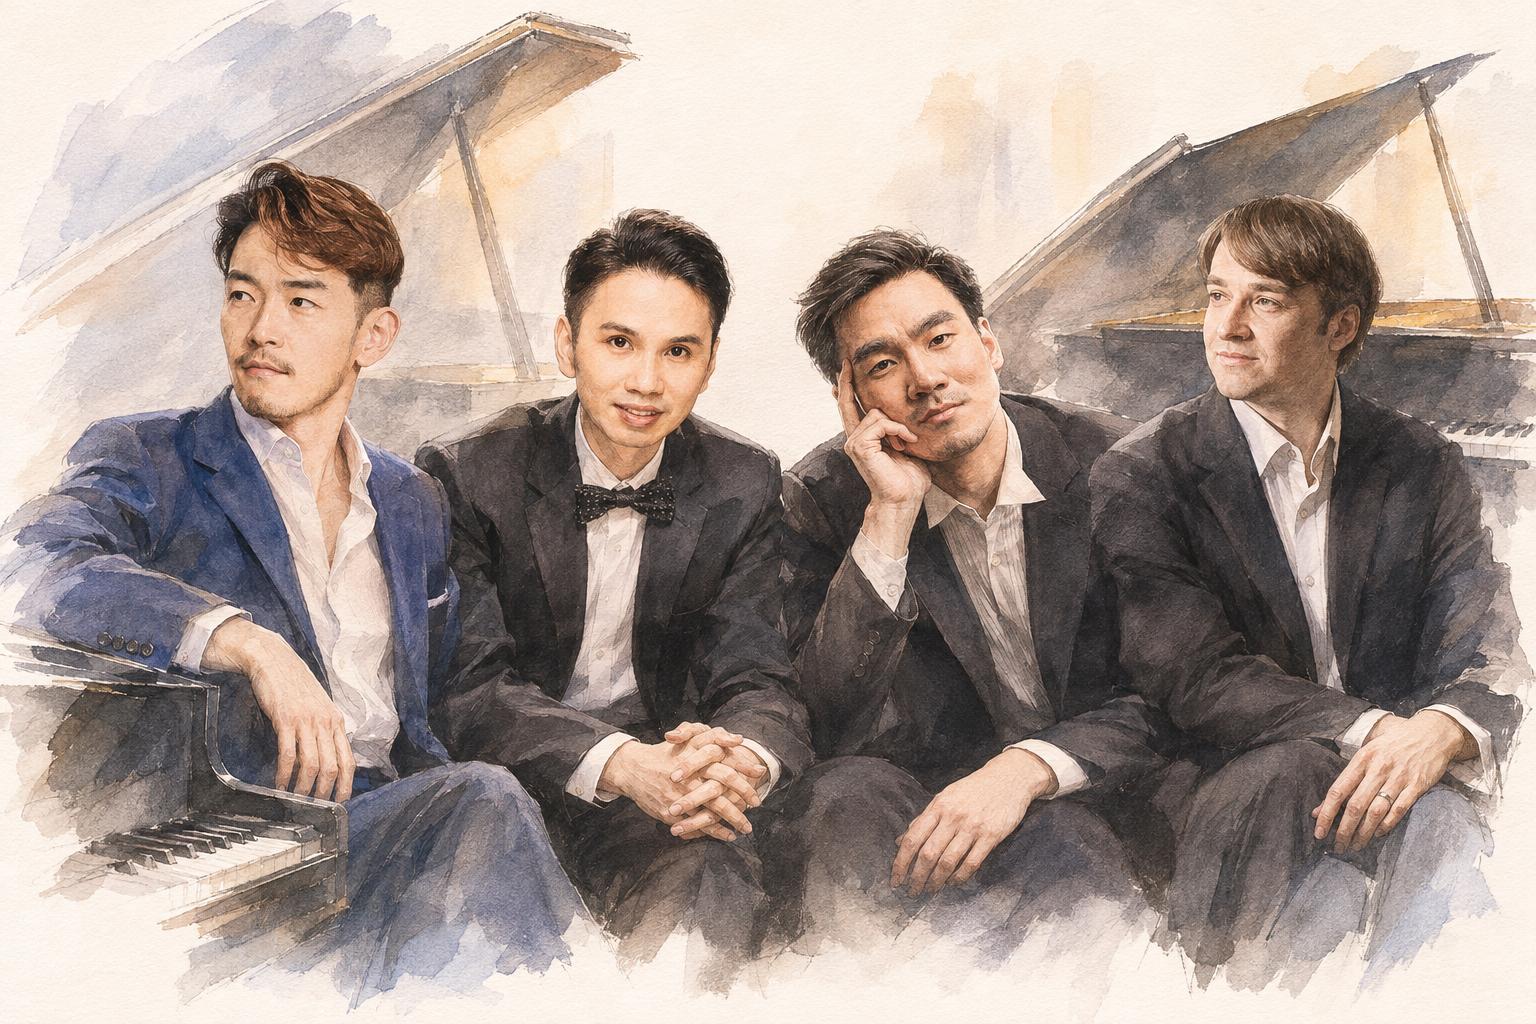
\includegraphics[width=0.95\textwidth]{Pianists.png}
  \par\smallskip
  {\small\color{accent} 四位演奏家的水彩素描：嚴俊傑、盧易之、汪奕聞與 Peter Ovcharov。}
  \par
  {\footnotesize 插畫依人物照片創作，非現場演出實況。}
\end{center}
\subsection{嚴俊傑｜Chun-Chieh Yen}
嚴俊傑曾於德國漢諾威隨 Vladimir Krainev 學習，並在美國 Colburn School 隨 John Perry 深造。他的演出兼及經典、新作與跨領域形式，曾與國家交響樂團錄製陳其鋼《二黃》，也策畫一天內三場不同主題獨奏會。其官方簡介列為國立臺灣師範大學鋼琴教授及國際大師鋼琴藝術節創辦人；史坦威臺灣於 2026 年公告他加入史坦威藝術家行列。\src{4,5}

\textbf{聆聽提示：} 留意樂句如何由輕到強地發展，以及旋律交給夥伴後，他如何調整音量與伴奏。

\subsection{盧易之｜Yi-Chih Lu}
盧易之求學於維也納音樂暨表演藝術大學與柏林藝術大學。除演奏蕭邦、布拉姆斯等曲目，他也長期投入臺灣作曲家作品與民謠改編。其創作活動橫跨獨奏、室內樂與合唱，適合從演奏、編曲與創作三個角度認識。2026 臺灣國際大提琴藝術節簡介列其為國立臺北藝術大學專任助理教授。\src{6}

\textbf{聆聽提示：} 可以先跟著較長的旋律，再聽伴奏如何襯托它；熟悉主題換到不同音域時，也留意觸鍵的變化。

\subsection{汪奕聞｜Evan Wong}
汪奕聞為第六屆仙台國際音樂大賽銀獎及觀眾獎得主，曾就讀新英格蘭音樂院、茱莉亞音樂學院、美國西北大學與漢諾威音樂戲劇媒體學院。他的演奏活動包括獨奏與室內樂，近年亦有全德布西節目，以及與張玹合作的《EARTHING》專輯。其官方簡介列為國立臺北藝術大學專任鋼琴教師。\src{7}

\textbf{聆聽提示：} 留意輕聲演奏時的旋律，以及兩台琴如何接續短音型、呼應節奏和音色。

\subsection{Peter Ovcharov｜亦見拼作 Peter Ovtcharov}
售票頁使用 Peter Ovcharov；奧地利 Allegro Vivo 音樂節等資料使用 Peter Ovtcharov。他曾於薩爾茲堡莫札特音樂大學隨 Karl-Heinz Kämmerling 學習，獲國際柴可夫斯基青少年比賽銀牌等獎項。Allegro Vivo 簡介列其為首爾延世大學鋼琴教授，並參與該音樂節的大師班教學，亦有與大提琴家 Adrian Brendel 等人的室內樂合作。\src{8}

\textbf{聆聽提示：} 除了快速音群，也可聽內聲與低音；兩台琴同時發聲時，留意各層聲部如何保持清楚。

{\small 各曲演奏搭檔請見現場節目單。}
\clearpage
\section{巴赫：先學會聽見多條旋律}
\work{約翰・塞巴斯蒂安・巴赫（1685--1750）}{Johann Sebastian Bach｜本場曲名、作品編號與改編者待公布}
巴赫是巴洛克時期重要的作曲家與鍵盤演奏者。他的音樂常讓數條各有方向的旋律同時進行：它們彼此模仿、交會，最後形成整體的秩序。這種寫法稱為對位；「複音」則強調同時存在多個相對獨立的聲部。

\subsection{從短音型認識對位}
可以先記住一個短音型的節奏和大致走向，再聽它是否換到另一個音域或另一台琴。即使無法辨認每個音，也能聽出相似的材料如何先後出現、互相模仿。

巴赫的低音也常有完整的旋律。高音很繁忙時，可以暫時聽聽低音如何移動、如何帶動和聲，再回到整體。這樣會比較容易分辨幾條旋律同時進行的關係。

\subsection{現代鋼琴帶來的選擇}
巴赫時代的鍵盤樂器與今日演奏型平台鋼琴不同。現代鋼琴提供寬廣的動態與延音，也使演奏者需要思考：如何使用踏板而不掩蓋線條，如何用音色區分聲部，如何兼顧舞曲的脈動與樂句的呼吸。

不同演奏者會採取不同做法。有的音較短，有的較連貫；只要音量和踏板控制得宜，都能讓聲部保持清楚。欣賞時，可以留意各條旋律是否容易分辨，以及節拍是否穩定。

\begin{listen}{可以試著這樣聽}
選一個短音型，聽它下一次出現在哪裡。接著把注意力轉到低音十幾秒，聽它是否也有連貫的旋律。
\end{listen}

\textbf{延伸聆聽：} 巴赫 C 小調雙大鍵琴協奏曲 BWV 1060，可用來認識兩件鍵盤樂器互相模仿的寫法。這首另有弦樂伴奏，並非本場已確認曲目。

\subsection{具名錄音與聆聽比對}
\textbf{鋼琴：Lucas Jussen、Arthur Jussen（尤森兄弟）；樂團：Amsterdam Sinfonietta；領奏：Candida Thompson。} 這份錄音以現代鋼琴演奏兩個鍵盤聲部，可以比較兩台琴如何互相模仿，以及如何與弦樂團交接。\src{28}

\begin{itemize}
\item \href{https://youtu.be/DBgV14408Q8}{聆聽：尤森兄弟演奏 BWV 1060 第一樂章 Allegro（官方音訊）}
\item \href{https://youtu.be/5ZUCSJfT0Ds}{聆聽：尤森兄弟演奏 BWV 1060 第二樂章 Adagio（官方音訊）}
\end{itemize}

第一樂章可追蹤兩台琴的動機接力；第二樂章則留意歌唱性的長句與伴奏如何保持呼吸。

\clearpage
\section{莫札特：D 大調雙鋼琴奏鳴曲 K.448}
\work{沃夫岡・阿瑪迪斯・莫札特（1756--1791）}{Wolfgang Amadeus Mozart｜Sonata for Two Pianos in D major, K.448}
\begin{center}
  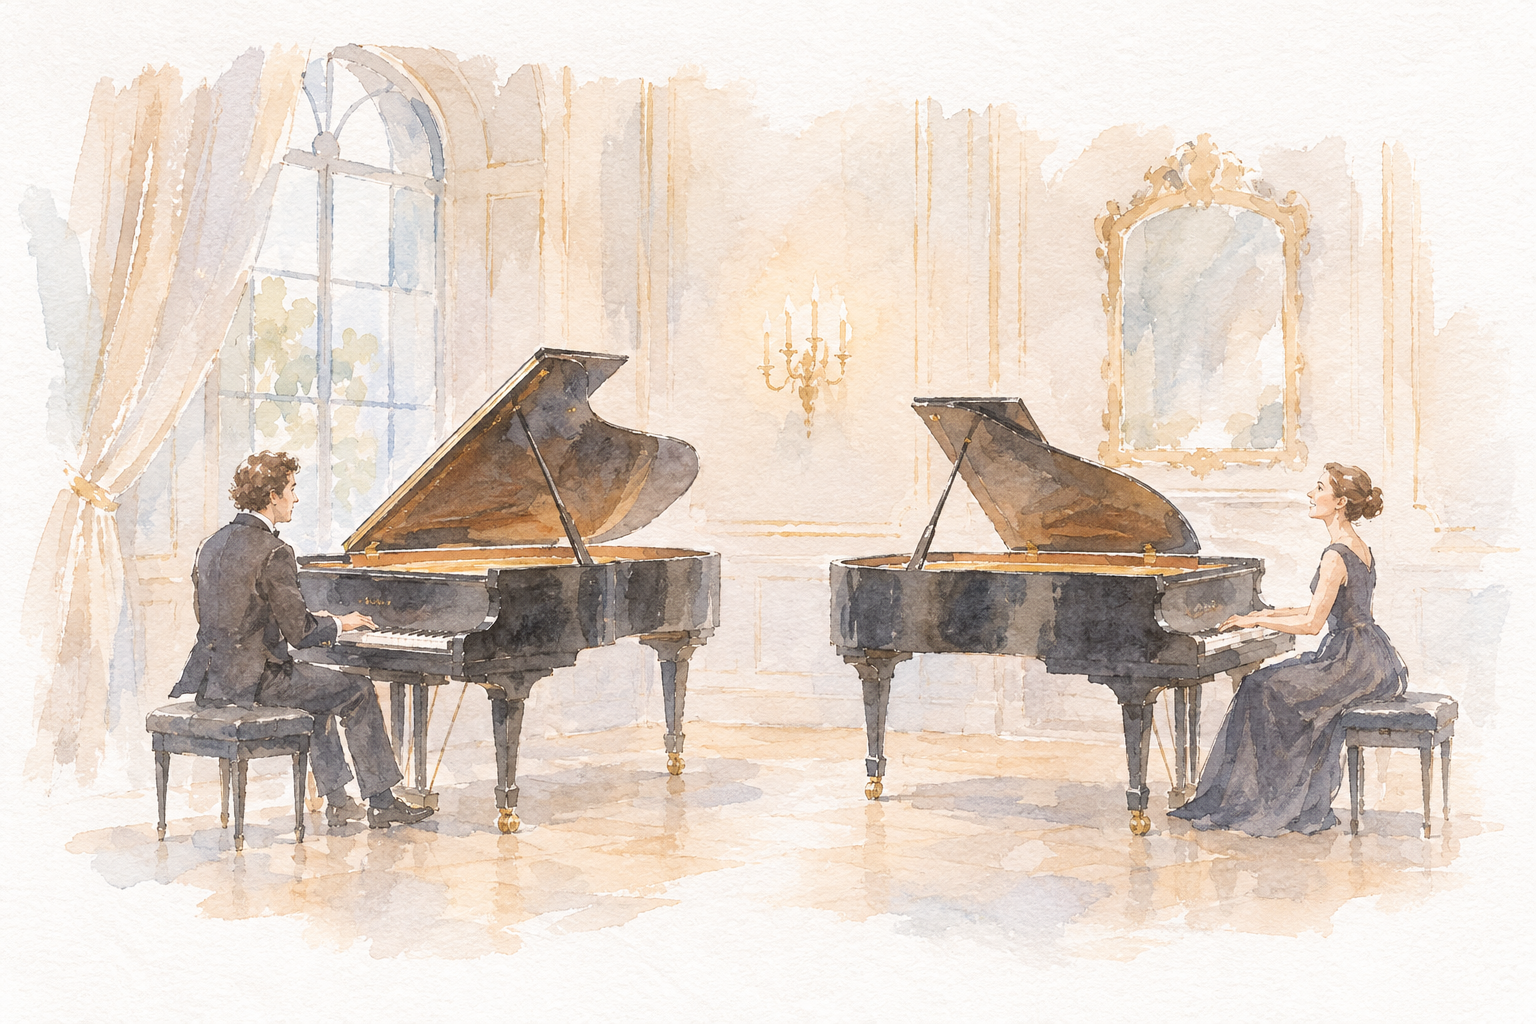
\includegraphics[width=0.72\textwidth]{Mozart_Two_Pianos.png}
\end{center}
這首奏鳴曲寫於 1781 年維也納時期，與鋼琴家 Josepha Auernhammer 的合作密切相關；莫札特基金會作品目錄記載，兩人於 1781 年 11 月 23 日在 Auernhammer 家演出。\src{9} 音樂裡的平衡感，來自兩台琴都能主動提出想法，又能迅速回應對方。

本曲包括三個樂章。以下介紹完整作品的走向；實際演出哪些樂章，以節目單為準。
\subsection{第一樂章：Allegro con spirito｜有精神的快板}
開頭由兩台琴一起奏出明亮、有力的樂句，隨後快速音型開始互相接續。有時兩台琴同時前進，有時輪流演奏。初次聽奏鳴曲式，可以先辨認主題出現、材料變化，以及熟悉主題回歸的幾個段落。

\textbf{聽點：} 聽快速音群換到另一台琴時，速度、力度和句尾是否接得自然。兩人同時演奏的段落，也可留意重音是否一致。

\subsection{第二樂章：Andante｜行板}
第二樂章速度放緩，旋律較為舒展。兩台琴輪流帶出主線，也分擔和聲與內聲。\src{10} 可以留意一句如何漸弱收尾，另一台琴又如何接續。

\textbf{聽點：} 彈伴奏的人如何控制音量，讓旋律清楚；旋律由高往低移動時，音色和力度又有什麼變化。

\subsection{第三樂章：Allegro molto｜很快的快板}
終樂章恢復明快的速度，主要主題多次出現，容易辨認。每次主題回來之前，都有不同的音型與段落，可以聽它們如何銜接，以及兩台琴如何保持輕巧的節奏。

\begin{listen}{清楚、輕巧的合奏}
莫札特的音符清楚，速度與力度的細微差異也容易聽見。可以留意兩人的起音、句尾和旋律交接，聽快速段落如何保持整齊，又不顯得僵硬。
\end{listen}

\begin{itemize}
  \item
  \href{https://www.youtube.com/watch?v=USl7qUWU33k}
  {名家演奏：阿格麗希與巴倫波因（EuroArts 公開影片）}

  \item
  \href{https://youtu.be/Cuit0WR_NYU}
{《交響情人夢》片段：莫札特雙鋼琴奏鳴曲 K.448，第一樂章}
\end{itemize}

\clearpage
\section{德布西：黑與白}
\work{克洛德・德布西（1862--1918）}{Claude Debussy｜En blanc et noir（1915）｜原為雙鋼琴而作}
\begin{center}
  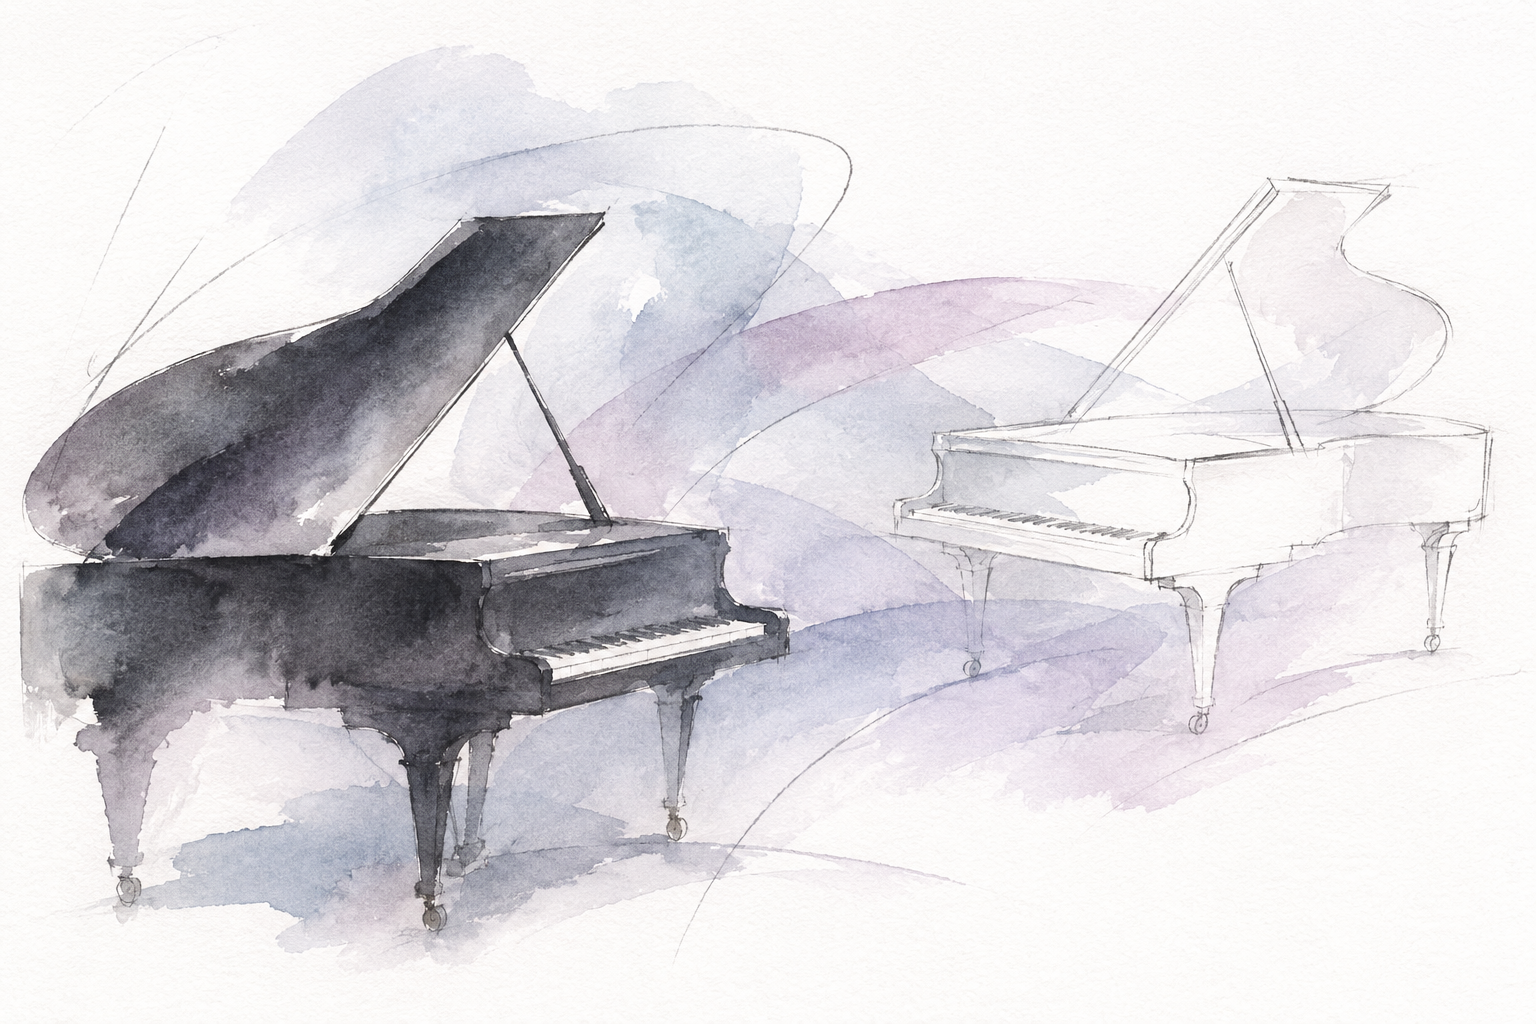
\includegraphics[width=0.72\textwidth]{Debussy_En_Blanc_Et_Noir.png}
\end{center}
德布西常以和聲、音域與觸鍵改變音色。《黑與白》寫於第一次世界大戰期間，三首樂曲的性格差異很大，從激烈的節奏到緩慢、沉重的段落都有。法國國家圖書館記載創作時間為 1915 年 6 月至 7 月，三首分別題獻給 Koussevitzky、Jacques Charlot 與史特拉汶斯基。\src{11}

曲名讓人聯想到鋼琴鍵盤，也適合用來注意音色的明暗對比。兩台琴有時分得很清楚，有時透過和聲與踏板的共鳴相互交疊；同樣的音型移到另一個音域，聽感也會改變。

\subsection{第一首：Avec emportement｜激昂地}
開頭節奏鮮明，音型快速交錯，重音也不斷移動。初次聽時，可以先跟著節奏，留意音域擴大、力度增強或突然收斂的地方，再慢慢辨認其中的旋律。

\textbf{聽點：} 同一類音型換到另一台琴時，音色有什麼不同；強奏之中，短音型和節奏是否仍清楚。

\subsection{第二首：Lent, sombre｜緩慢、陰暗地}
第二首紀念在戰爭中陣亡的 Jacques Charlot，速度較慢，氣氛沉重。\src{12} 低音、停頓與突然出現的強音形成明顯對比，可以留意它們之間的間隔，以及和聲遲遲未解決時的緊張感。

\textbf{聽點：} 有些段落雖然很輕，和聲卻仍緊張。聽停頓前後的音量與音域變化，會更容易掌握這首的起伏。

\subsection{第三首：Scherzando｜詼諧地}
第三首題獻給史特拉汶斯基，音樂短促、敏捷，節奏變化也多。可以追蹤簡短動機在兩台琴之間如何接續、重複和改變，聽它們如何組成較長的段落。

\begin{listen}{踏板與音色的變化}
留意哪些聲音相連，哪些地方收得乾淨。踏板讓和聲產生共鳴，也可能使不同聲部重疊；兩位演奏者需要協調延音和收音，才能兼顧音色與清晰度。
\end{listen}
 
\noindent
\href{https://youtu.be/HHZ3RYAHq20}
{德布西《黑與白》雙鋼琴：阿格麗希與伊多・巴爾夏伊（Martha Argerich \& Iddo Bar-Shai）}

\medskip

\noindent
\href{https://www.youtube.com/results?search_query=Debussy+En+blanc+et+noir+Argerich+Kovacevich}
{YouTube 搜尋：阿格麗希與柯瓦謝維契《黑與白》}

\clearpage
\section{拉威爾：圓舞曲}
\work{莫里斯・拉威爾（1875--1937）}{Maurice Ravel｜La Valse（1920）｜雙鋼琴版本}
\begin{center}
  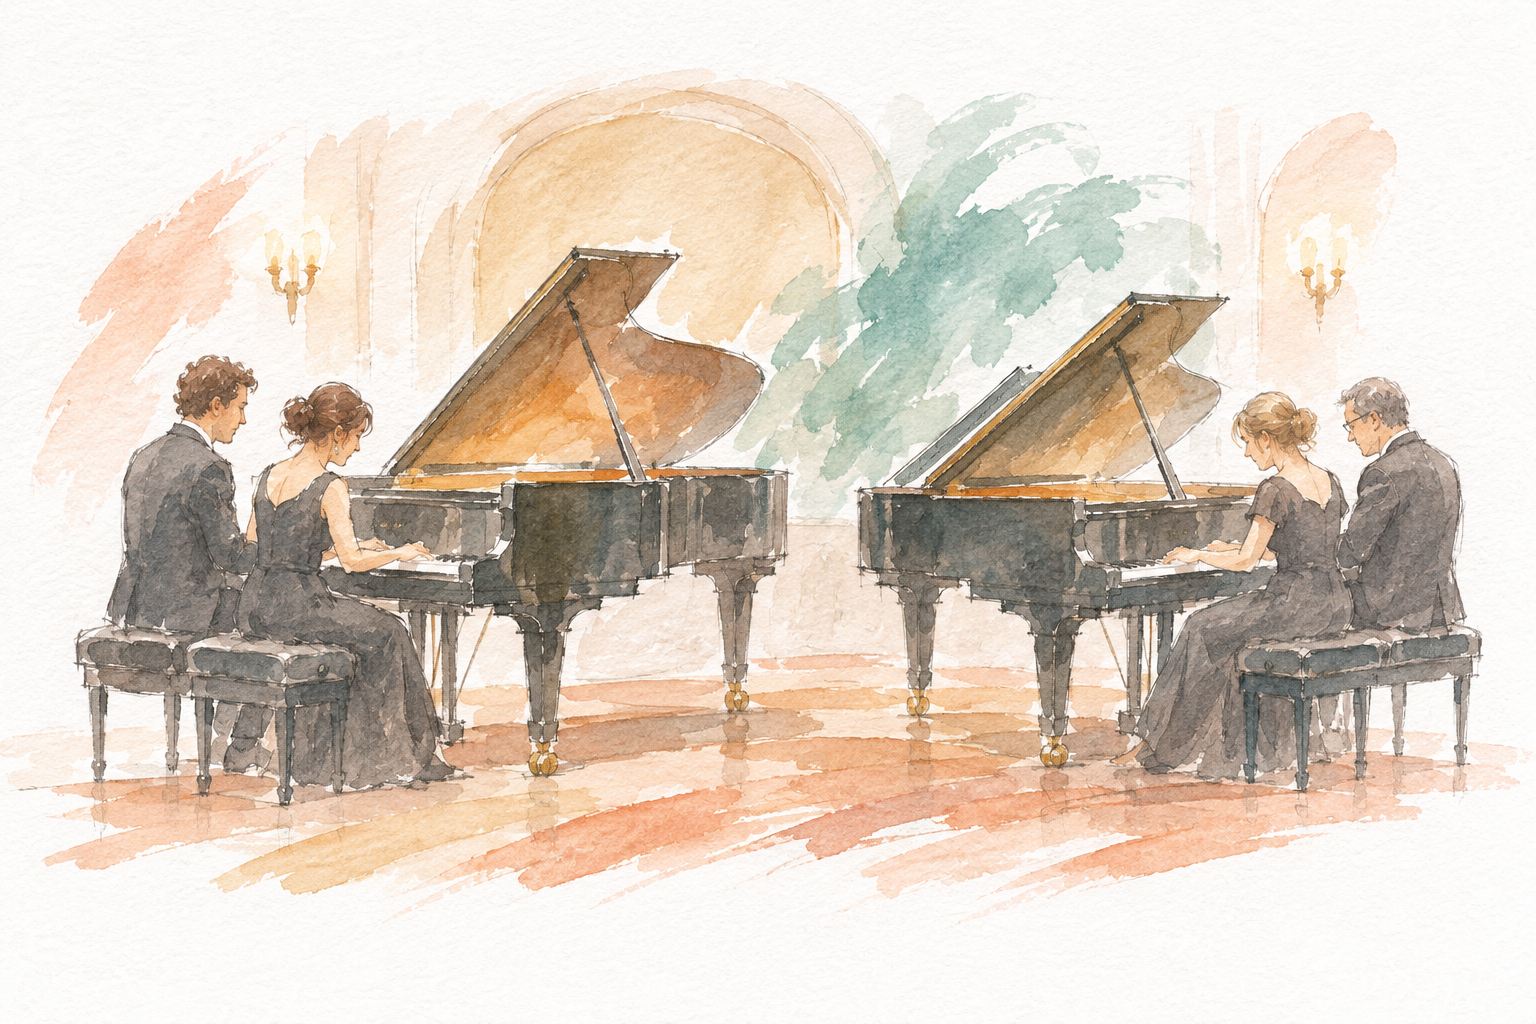
\includegraphics[width=0.72\textwidth]{Ravel_La_Valse.png}
\end{center}
拉威爾長期對維也納圓舞曲有興趣，《圓舞曲》於 1920 年完成，有管弦樂、鋼琴獨奏與雙鋼琴等版本。\src{13} 雙鋼琴版少了管弦樂器的音色區別，卻讓三拍子的節奏、低音與快速音群更容易辨認。

\subsection{開場：逐漸清楚的三拍子}
開頭先出現低音與零碎的舞曲片段，三拍子逐漸清楚，完整旋律才慢慢出現。拉威爾在手稿中描寫雲霧散開、舞廳浮現的場景，並註明約 1855 年的帝國宮廷。\src{14}

\textbf{聽點：} 旋律尚未完整出現時，先找三拍子的節奏，聽低音與短音型如何讓舞曲逐漸成形。

\subsection{中段：旋律與舞曲節奏}
旋律清楚之後，兩台琴輪流演奏不同的舞曲主題，並分擔低音與和聲。除了主要旋律，也可以聽伴奏的重音和內聲，它們讓三拍子持續前進，並帶出不同段落的變化。

\subsection{後段：聲響與節奏的累積}
後段的音符越來越密集，重音更加突出，速度感也更強。同樣的三拍子從輕快逐漸變得急促，兩台琴的聲響不斷加厚，直到強烈的結尾。

作品常被解讀為戰後對舊歐洲的回望，但音樂本身並沒有唯一的故事。聆聽時，可以直接追蹤節奏、重音與力度的變化，感受圓舞曲的性格如何逐漸改變。

\begin{listen}{本曲最值得追蹤的變化}
從開頭到結尾，留意三拍子的重音如何變化。音符越來越多時，也可聽兩台琴如何分配旋律、低音與和聲，讓音樂仍有清楚的層次。
\end{listen}

\href{https://www.youtube.com/watch?v=Q0Qo1anGvfQ}{試聽：阿格麗希與 Nelson Freire，拉威爾《圓舞曲》雙鋼琴版}

\clearpage
\section{土耳其狂想曲：八手聯彈的主題變化}
\work{《土耳其狂想曲》｜八手聯彈}{Turkish Rhapsody｜本場作者、改編者與素材來源待確認}
\begin{center}
  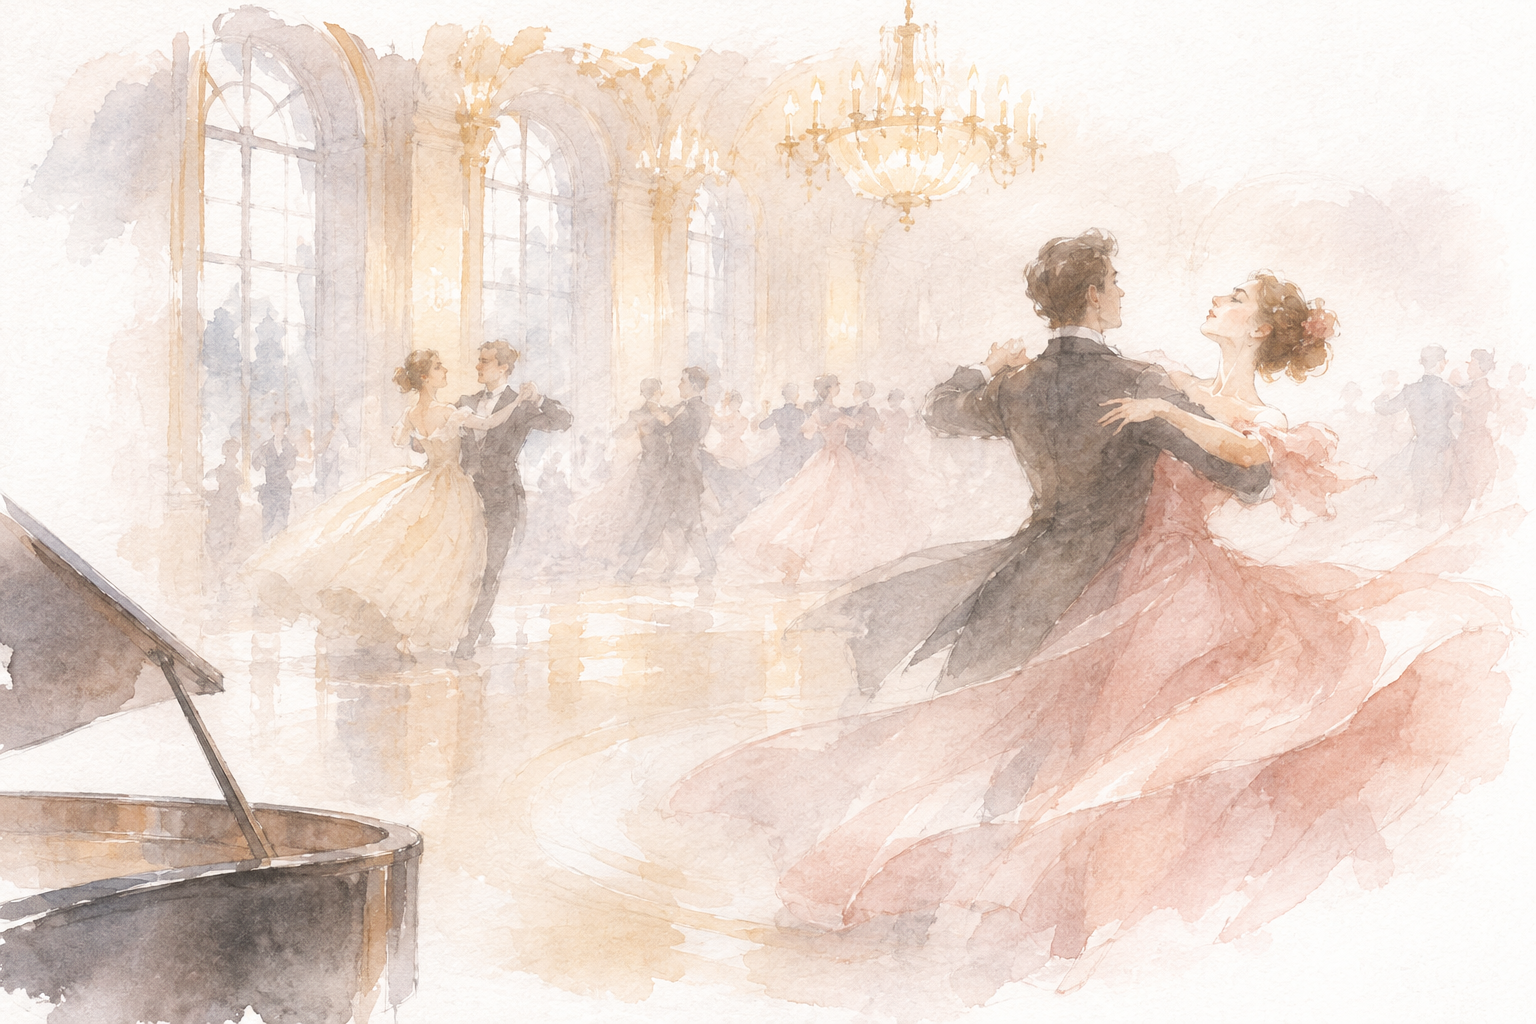
\includegraphics[width=0.72\textwidth]{Turkish_Rhapsody.png}
\end{center}
本場售票頁列出《土耳其狂想曲》及八手聯彈的編制，作者與改編者尚待正式節目單確認。\src{1}

\subsection{改編版本與具名演出資料}
其他音樂會曾演出署名 W. A. Mozart / V. Gryaznov 的《土耳其狂想曲》，編制為兩台鋼琴八手；首爾藝術殿堂等節目資料可見這個版本。\src{15} 以下將它作為延伸參考，新竹場是否使用同一版仍待確認。

\subsection{如果主題來自莫札特的土耳其風格}
莫札特 A 大調鋼琴奏鳴曲 K.331 的終樂章標作 Alla turca，是最熟悉的土耳其風格鍵盤音樂之一。這類語彙反映十八世紀歐洲對鄂圖曼軍樂的想像，常藉鮮明節奏與打擊感營造熱鬧氣氛。若現場作品使用這個素材，可以留意熟悉旋律如何被擴展，而非只等待原曲原樣重現。

狂想曲的段落通常較自由，也常安排炫技效果。改編者可以更換音域、節奏、和聲與聲部分配，讓同一個主題有時由少數聲部演奏，有時由四人一起奏出。

\begin{listen}{八手聯彈的聽點}
\begin{itemize}
\item 主題由誰演奏，其他人如何以低音、和聲或節奏配合。
\item 熟悉的旋律如何被延長、拆分，或移到低音。
\item 突然停頓後，四人如何一起重新進入。
\item 高潮音符密集時，主題是否仍然清楚。
\end{itemize}
\end{listen}

\textbf{延伸演出資料：王旼、邱琳云、陳威存、蘇品諼。} OPENTIX「琴弦狂舞 2.0—鋼琴重奏音樂會」列有這四位鋼琴家，以及 Mozart / Gryaznov《土耳其狂想曲》雙鋼琴八手版。以下連結為該場節目介紹。\src{29}

\noindent
\href{https://www.opentix.life/event/2011709863623639041}{查看「琴弦狂舞 2.0」曲目及四位鋼琴家名單}

上述連結可查看曲名、編制與演奏者，並非演出影片。

\clearpage
\section{聖桑：骷髏之舞}
\work{卡米爾・聖桑（1835--1921）}{Camille Saint-Saëns｜Danse macabre, Op.40｜本場為八手改編}
\begin{center}
  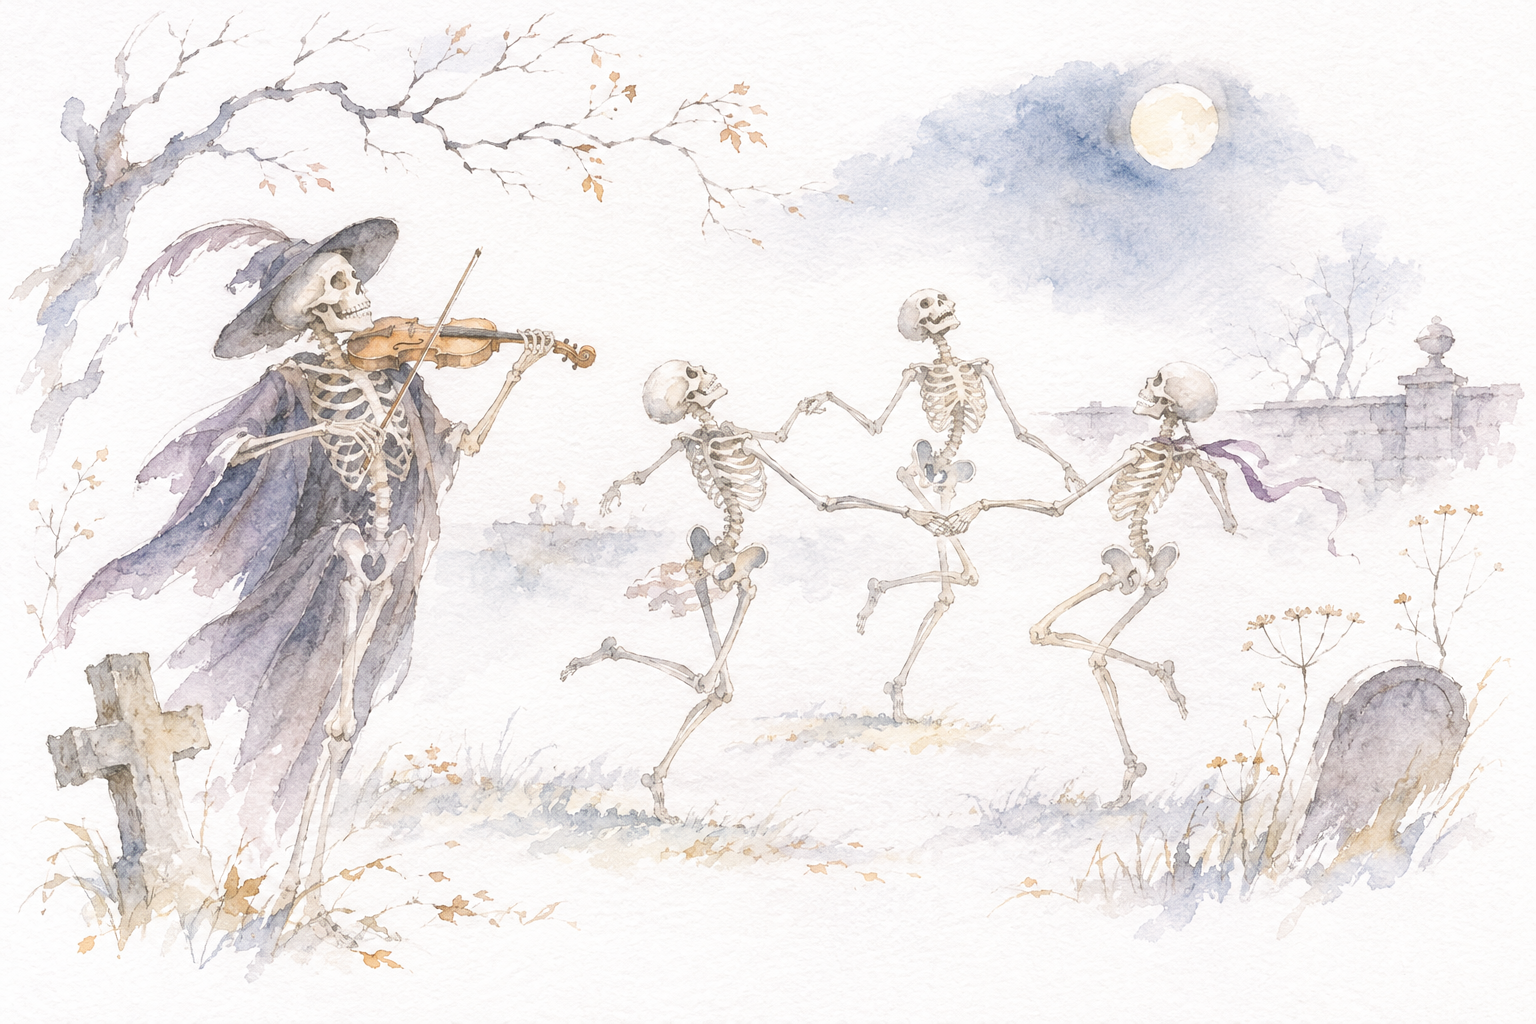
\includegraphics[width=0.72\textwidth]{Saint_Saens_Danse_Macabre.png}
\end{center}
聖桑的音樂常把精密技巧與鮮明形象結合。《骷髏之舞》先有 1872 年的歌曲版本，後發展為 1874 年的交響詩。故事描繪午夜時死神拉起小提琴，召喚骷髏跳舞，直到雞啼、天亮，舞群才退回墓穴。\src{16}

\subsection{故事的幾個聲音標記}
在管弦樂版中，開頭豎琴反覆奏出的音代表午夜十二下鐘聲；獨奏小提琴的尖銳音程讓死神現身。木琴則以乾脆的敲擊感描寫骨骼碰撞，最後由雙簧管帶出雞啼的訊號。\src{16}

八手改編把這些管弦樂效果交給鋼琴。演奏者透過不同音域、長短不一的觸鍵與聲部安排，區分鐘聲、旋律和短促的敲擊聲。先聽過管弦樂版，再聽鋼琴合奏，會更容易辨認這些細節。

\subsection{舞曲中的緊張與幽默}
《骷髏之舞》雖然描寫死亡，節奏卻相當活潑。穩定的舞曲中，不時出現尖銳、短促或突然加強的聲音，讓音樂同時帶有緊張和詼諧的效果。

\subsection{改編者帶來的差異}
Ernest Guiraud 曾將這首作品改編為兩台鋼琴八手，Durand／Hal Leonard 有出版樂譜。\src{17} 本場的改編者尚未公布；不同版本的聲部分配與演奏效果也可能不同。

\begin{listen}{把鋼琴聽成不同的樂器}
短而清脆的高音容易讓人聯想到骨骼碰撞，延展的旋律則承接原作小提琴的部分。可以聽這兩類聲音如何交錯，以及接近結尾時，聲部如何逐漸減少、音量如何收下來。
\end{listen}

\subsection{具名演奏版本與聆聽比對}
\textbf{鋼琴合奏：今野早苗、菅生晴美、前場央子、前場聖子。} 日本鋼琴教師協會 PTNA 收錄這四位鋼琴家於 2017 年 4 月 15 日的錄影，可用來觀察多人合作的聲部分工。\src{30}

\noindent
\href{https://youtu.be/E2cIH5tMAoA}{觀看演出：《骷髏之舞》——今野早苗、菅生晴美、前場央子、前場聖子}

\medskip
\textbf{管弦樂版：Empyrean Orchestra；指揮：Kevin Griffiths；小提琴獨奏：Sherniyaz Mussakhan。} 樂團官方影音頁列出這場演出的完整陣容。\src{31}

\noindent
\href{https://youtu.be/LxKQpEVYWog}{觀看演出：《骷髏之舞》管弦樂版——Kevin Griffiths 指揮、Sherniyaz Mussakhan 小提琴獨奏}

\begin{listen}{兩種編制如何描寫同一場夜舞}
先聽管弦樂版的午夜鐘聲、小提琴與木琴，再聽鋼琴合奏如何以不同音域、短促觸鍵及聲部配置塑造相近的形象。比較時也留意旋律的突出程度、舞曲的脈動，以及高潮過後聲音如何轉薄。
\end{listen}

\clearpage
\section{拉赫曼尼諾夫：風格與延伸聆聽}
\work{謝爾蓋・拉赫曼尼諾夫（1873--1943）}{Sergei Rachmaninoff｜公開介紹提及作曲家，未列本場曲名}
拉赫曼尼諾夫同時是作曲家與傑出的鋼琴家。他的鋼琴音樂常以寬廣的旋律、豐厚的和聲與深沉低音著稱。遇到多層次的織度時，不必試著追逐所有音符；先抓住旋律，再聽內聲與低音如何讓它逐步累積情緒。

在雙鋼琴作品中，寬廣旋律、厚重低音與快速音群可以由兩人分擔。聽高潮段落時，可以留意旋律是否持續突出，以及伴奏如何逐步增加音量與密度。

\begin{listen}{兩首延伸作品}
《第二號雙鋼琴組曲》Op.17 與《交響舞曲》Op.45 雙鋼琴版，都是認識拉赫曼尼諾夫的合適選擇。本場尚未公布他的曲名，這裡先作為延伸欣賞。
\end{listen}

\subsection{具名演奏版本與延伸聆聽}
\begin{itemize}
\item \textbf{《第二號組曲》Op.17：阿格麗希與 Nelson Freire。}
\href{https://youtu.be/wYLasmJdeEg}{觀看演出：Martha Argerich \& Nelson Freire}
\item \textbf{《交響舞曲》Op.45 雙鋼琴版：阿格麗希與 Nelson Goerner。}
\href{https://vimeo.com/27052613}{觀看演出節錄：Martha Argerich \& Nelson Goerner，2011 年韋爾比耶音樂節}
\end{itemize}

這兩段錄影的搭檔不同。聆聽時可分別追蹤長旋律如何接續、低音如何推動節奏，以及兩台琴如何在高潮中保持聲部層次；兩首作品的概覽另見第 \ref{sec:duo-videos} 節的影音表格。

\subsection{把三種聲音世界放在一起聽}
比較幾位作曲家時，可以從不同細節開始：莫札特先聽樂句的交接，德布西留意和聲與共鳴，拉赫曼尼諾夫則跟著長旋律和低音。熟悉之後，再聽其他聲部會更容易。

\subsection{現場補記}
正式曲名與作品編號：\hrulefill\par\vspace{0.4cm}
演出者／搭檔：\hrulefill\par\vspace{0.4cm}
最想回家再聽的一段：\hrulefill
\clearpage
\section{試聽路線與現場筆記}
\subsection{三十分鐘的預習安排}
\begin{enumerate}[leftmargin=*,itemsep=5pt]
\item \textbf{莫札特，約八分鐘：} 聽第一樂章開頭與第二樂章一段，熟悉清楚的雙鋼琴對話。
\item \textbf{德布西，約七分鐘：} 各聽第一、第二首的一段，比較快速交錯與緩慢沉重的段落。
\item \textbf{拉威爾，約十分鐘：} 盡量連續聽，聽三拍子如何逐漸清楚，以及後段聲響如何加厚。
\item \textbf{八手，約五分鐘：} 選一段《骷髏之舞》八手演出，看四人的合作與聲部分工。
\end{enumerate}
以上是預習時間分配，不是作品長度或本場演出時間。

\subsection{試聽連結的使用方式}
本手冊在曲目導聆與延伸表格中提供直接影音連結，包括莫札特 K.448、德布西《黑與白》、拉赫曼尼諾夫《第二號組曲》及拉威爾《圓舞曲》；《交響舞曲》則提供 medici.tv 公開的演出節錄。另有《交響情人夢》片段，方便比較戲劇場景與音樂會演出。標成「YouTube 搜尋」的連結是搜尋入口，結果會變動，請依曲名、演奏者及編制辨認。

請先確認畫面或說明是否寫明 \textit{two pianos}；八手作品則找 \textit{two pianos, eight hands}。與現場相比時，先確認演出編制及是否為全曲或節錄。影片中的演奏家是預習參考，並非本場陣容。

\begin{listen}{演後筆記}
\textbf{印象深刻的音色或段落：}\par\vspace{0.3cm}
\hrulefill\par
\textbf{值得記下的旋律交接或共同收尾：}\par\vspace{0.3cm}
\hrulefill\par
\textbf{想再聽的作品與原因：}\par\vspace{0.3cm}
\hrulefill
\end{listen}
\subsection{安可曲｜Encores（演後填寫）}
本手冊不預設安可曲目。\par
1.\ 曲名／作曲家：\hrulefill\par\vspace{0.2cm}
2.\ 曲名／作曲家：\hrulefill
\clearpage
\section{資料來源與版本說明}
{\small 本手冊為個人聆聽導引，非主辦單位正式節目冊。音樂的畫面描述與可以試著這樣聽為導聆建議；生平、作品年代及公開節目資訊依下列資料整理。查核日期：2026 年 11 月 1 日。}
\begin{enumerate}[label={[\arabic*]},leftmargin=*,itemsep=6pt,font=\small]

\item OPENTIX：2026 黑白極致・巨擘對話—名家音樂會。 \href{https://www.opentix.life/event/2089958531710963713}{開啟來源}

\item Steinway \& Sons：D-274 官方規格。 \href{https://eu.steinway.com/en/pianos/grand-pianos/d-274}{開啟來源}

\item 風城演藝：2026 年 10 月 2 日選琴公告（依公告截圖整理）。

\item 嚴俊傑官方網站：Biography。 \href{https://www.chunchiehyen.com/biography}{開啟來源}

\item 史坦威臺灣：2026 年 4 月 29 日嚴俊傑加入史坦威藝術家公告。 \href{https://www.steinway.com.tw/news/steinway-news/20260429-Steinway-Artist-Prof.-Yen-Chun-Chieh.}{開啟來源}

\item 2026 臺灣國際大提琴藝術節：盧易之介紹。 \href{https://www.twicf.org/artist/\%E7\%9B\%A7\%E6\%98\%93\%E4\%B9\%8B-yi-chih-lu}{開啟來源}

\item 汪奕聞官方網站：About Evan。 \href{https://www.evanwongpiano.com/bio?lang=zh}{開啟來源}

\item Allegro Vivo：Peter Ovtcharov 藝術家介紹。 \href{https://www.allegro-vivo.at/en/artist/peter-ovtcharov/}{開啟來源}

\item 莫札特基金會 Köchel 作品目錄：KV 448。 \href{https://kv.mozarteum.at/en/work/sonata-in-d-for-2-keyboard-instruments-4748}{開啟來源}

\item 洛杉磯愛樂：Sonata in D Major for Two Pianos, K.448。 \href{https://www.laphil.com/works/sonata-in-d-major-for-two-pianos-k-448}{開啟來源}

\item 法國國家圖書館：En blanc et noir 作品目錄。 \href{https://catalogue.bnf.fr/ark:/12148/cb13911379p}{開啟來源}

\item Gerald Larner 導聆檔案：En blanc et noir (1915)。 \href{https://geraldlarner.com/work/debussy-en-blanc-et-noir-1915}{開啟來源}

\item 洛杉磯愛樂：La valse for two pianos。 \href{https://www.laphil.com/works/la-valse-for-two-pianos}{開啟來源}

\item Morgan Library：La valse 雙鋼琴手稿。 \href{https://www.themorgan.org/music-manuscripts-and-printed-music/115543}{開啟來源}

\item 首爾藝術殿堂：其他音樂會的 Mozart / Gryaznov 八手節目紀錄，僅作版本線索。 \href{https://www.sac.or.kr/site/main/show/show_view?SN=37377\&tab=5}{開啟來源}

\item 美國國會圖書館：Saint-Saëns and Danse macabre。 \href{https://blogs.loc.gov/nls-music-notes/2022/10/song-stories-camille-saint-sans-and-danse-macabre/}{開啟來源}

\item Hal Leonard／Durand：Danse macabre 兩琴八手版，Guiraud 改編。 \href{https://www.halleonard.com/product/50561382/danse-macabre-op-40-poeme-symphonique}{開啟來源}

\item EuroArts YouTube：阿格麗希與巴倫波因演出 K.448。 \href{https://www.youtube.com/watch?v=USl7qUWU33k}{開啟來源}

\item YouTube：阿格麗希與 Nelson Freire 演出《圓舞曲》雙鋼琴版。 \href{https://www.youtube.com/watch?v=Q0Qo1anGvfQ}{開啟來源}

\item medici.tv：阿格麗希與巴倫波因於柯隆劇院的德布西等曲目演出。 \href{https://www.medici.tv/en/others/martha-argerich-and-daniel-barenboim-piano-duos-teatro-colon}{開啟來源}

\item 阿格麗希藝術基金會：Martha Argerich 官方簡介。\href{https://argerich-mf.jp/en/artist/martha-argerich}{開啟來源}

\item Warner Classics：《Music for Two Pianos》，盧加諾合作錄音選輯。\href{https://www.warnerclassics.com/release/music-two-pianos}{開啟來源}

\item 多倫多大學音樂學院：Bachelor of Music, Composition 課程。\href{https://music.utoronto.ca/programs/undergraduate/classical/composition}{開啟來源}

\item 奧勒岡大學：Piano Proficiency Exam for Composition Majors。\href{https://musicanddance.uoregon.edu/piano-proficiency-exam-composition-majors}{開啟來源}

\item G. Henle：貝多芬《第四號鋼琴協奏曲》Op.58，雙鋼琴縮譜版本。\href{https://www.henle.de/Piano-Concerto-no.-4-G-major-op.-58/HN-629}{開啟來源}

\item medici.tv：阿格麗希與 Nelson Goerner 演出《交響舞曲》，2011 年韋爾比耶音樂節節錄。\href{https://vimeo.com/27052613}{開啟影片}

\item YouTube：阿格麗希與 Nelson Freire 演出《第二號組曲》Op.17。\href{https://youtu.be/wYLasmJdeEg}{開啟影片}

\item Lucas \& Arthur Jussen 官方藝人頻道：巴赫 BWV 1060 第一、第二樂章，雙鋼琴與 Amsterdam Sinfonietta。\href{https://youtu.be/DBgV14408Q8}{第一樂章音訊}；\href{https://youtu.be/5ZUCSJfT0Ds}{第二樂章音訊}

\item OPENTIX：「琴弦狂舞 2.0—鋼琴重奏音樂會」，演奏者王旼、邱琳云、陳威存、蘇品諼；節目列有 Mozart / Gryaznov《土耳其狂想曲》。\href{https://www.opentix.life/event/2011709863623639041}{開啟演出資料}

\item 日本鋼琴教師協會 PTNA：《骷髏之舞》作品及影片資料；今野早苗、菅生晴美、前場央子、前場聖子，2017 年 4 月 15 日錄音。\href{https://enc.piano.or.jp/musics/3029}{開啟來源}；\href{https://youtu.be/E2cIH5tMAoA}{觀看影片}

\item Empyrean Orchestra 官方影音頁：《骷髏之舞》，Kevin Griffiths 指揮，Sherniyaz Mussakhan 小提琴獨奏。\href{https://empyreanorchestra.com/en/videos}{開啟來源}；\href{https://youtu.be/LxKQpEVYWog}{觀看影片}

\end{enumerate}
\end{document}
